%% abtex2-modelo-relatorio-tecnico.tex, v-1.9.7 laurocesar
%% Copyright 2012-2018 by abnTeX2 group at http://www.abntex.net.br/ 
%%
%% This work may be distributed and/or modified under the
%% conditions of the LaTeX Project Public License, either version 1.3
%% of this license or (at your option) any later version.
%% The latest version of this license is in
%%   http://www.latex-project.org/lppl.txt
%% and version 1.3 or later is part of all distributions of LaTeX
%% version 2005/12/01 or later.
%%
%% This work has the LPPL maintenance status `maintained'.
%% 
%% The Current Maintainer of this work is the abnTeX2 team, led
%% by Lauro César Araujo. Further information are available on 
%% http://www.abntex.net.br/
%%
%% This work consists of the files abntex2-modelo-relatorio-tecnico.tex,
%% abntex2-modelo-include-comandos and abntex2-modelo-references.bib
%%

% ------------------------------------------------------------------------
% ------------------------------------------------------------------------
% abnTeX2: Modelo de Relatório Técnico/Acadêmico em conformidade com 
% ABNT NBR 10719:2015 Informação e documentação - Relatório técnico e/ou
% científico - Apresentação
% ------------------------------------------------------------------------ 
% ------------------------------------------------------------------------

\documentclass[
	% -- opções da classe memoir --
	12pt,				% tamanho da fonte
	openany,			% capítulos começam em pág ímpar (insere página vazia caso preciso)
	oneside,			% para impressão em recto e verso. Oposto a oneside
	a4paper,			% tamanho do papel. 
	% -- opções da classe abntex2 --
	%chapter=TITLE,		% títulos de capítulos convertidos em letras maiúsculas
	%section=TITLE,		% títulos de seções convertidos em letras maiúsculas
	%subsection=TITLE,	% títulos de subseções convertidos em letras maiúsculas
	%subsubsection=TITLE,% títulos de subsubseções convertidos em letras maiúsculas
	% -- opções do pacote babel --
	english,			% idioma adicional para hifenização
	french,				% idioma adicional para hifenização
	spanish,			% idioma adicional para hifenização
	brazil,				% o último idioma é o principal do documento
	]{abntex2}

%\documentclass[12pt,a4paper,openany,oneside]{abntex2}
% ---
% PACOTES
% ---

% ---
% Pacotes fundamentais 
% ---
\usepackage{lmodern}			% Usa a fonte Latin Modern
\usepackage[T1]{fontenc}		% Selecao de codigos de fonte.
\usepackage[utf8]{inputenc}		% Codificacao do documento (conversão automática dos acentos)
\usepackage{indentfirst}		% Indenta o primeiro parágrafo de cada seção.
\usepackage{color}				% Controle das cores
\usepackage{graphicx}			% Inclusão de gráficos
\usepackage{microtype} 			% para melhorias de justificação
\usepackage{nameref}
\usepackage{chngcntr}
\usepackage{amsmath}            % para escrever matrizes
\counterwithin{equation}{chapter}
\counterwithin{figure}{chapter}
\counterwithin{table}{chapter}
% ---

% ---
% Pacotes adicionais, usados no anexo do modelo de folha de identificação
% ---
\usepackage{multicol}
\usepackage{multirow}
% ---
	
% ---
% Pacotes adicionais, usados apenas no âmbito do Modelo Canônico do abnteX2
% ---
\usepackage{lipsum}				% para geração de dummy text
% ---

% ---
% Pacotes de citações
% ---
\usepackage[brazilian,hyperpageref]{backref}	 % Paginas com as citações na bibl
\usepackage[alf]{abntex2cite}	% Citações padrão ABNT

% --- 
% CONFIGURAÇÕES DE PACOTES
% --- 

% ---
% Configurações do pacote backref
% Usado sem a opção hyperpageref de backref
\renewcommand{\backrefpagesname}{Citado na(s) página(s):~}
% Texto padrão antes do número das páginas
\renewcommand{\backref}{}
% Define os textos da citação
\renewcommand*{\backrefalt}[4]{
	\ifcase #1 %
		Nenhuma citação no texto.%
	\or
		Citado na página #2.%
	\else
		Citado #1 vezes nas páginas #2.%
	\fi}%
% ---

% ---
% Informações de dados para CAPA e FOLHA DE ROSTO
% ---
\titulo{Controle no Espaço de Estados}
\autor{José E. de A. Junior: 20170009356\\
\vspace{0.8cm}
Kallil de A. Bezerra: 20180154987\\
\vspace{0.8cm}
Rafael de M. M. Capuano: 20180010172\\
\vspace{0.8cm}
Victor K. C. Sousa: 20180155278\\}
\local{Brasil}
\data{Dezembro de 2020}
\instituicao{%
  Universidade Federal do Rio Grande do Norte -- UFRN
  \par
  Departamento de Engenharia da Computação e Automação -- DCA}
\tipotrabalho{Relatório técnico}
% O preambulo deve conter o tipo do trabalho, o objetivo, 
% o nome da instituição e a área de concentração 
\preambulo{Modelo canônico de Relatório Técnico e/ou Científico em conformidade
com as normas ABNT apresentado à comunidade de usuários \LaTeX.}
% ---

% ---
% Configurações de aparência do PDF final

% alterando o aspecto da cor azul
\definecolor{blue}{RGB}{41,5,195}

% informações do PDF
\makeatletter
\hypersetup{
     	%pagebackref=true,
		pdftitle={\@title}, 
		pdfauthor={\@author},
    	pdfsubject={\imprimirpreambulo},
	    pdfcreator={LaTeX with abnTeX2},
		pdfkeywords={abnt}{latex}{abntex}{abntex2}{relatório técnico}, 
		colorlinks=true,       		% false: boxed links; true: colored links
    	linkcolor=blue,          	% color of internal links
    	citecolor=blue,        		% color of links to bibliography
    	filecolor=magenta,      		% color of file links
		urlcolor=blue,
		bookmarksdepth=4
}
\makeatother
% --- 

% --- 
% Espaçamentos entre linhas e parágrafos 
% --- 

% O tamanho do parágrafo é dado por:
\setlength{\parindent}{1.3cm}

% Controle do espaçamento entre um parágrafo e outro:
\setlength{\parskip}{0.2cm}  % tente também \onelineskip

% ---
% compila o indice
% ---
\makeindex
% ---

% ----
% Início do documento
% ----
\begin{document}

% Seleciona o idioma do documento (conforme pacotes do babel)
%\selectlanguage{english}
\selectlanguage{brazil}

% Retira espaço extra obsoleto entre as frases.
\frenchspacing 

% ----------------------------------------------------------
% ELEMENTOS PRÉ-TEXTUAIS
% ----------------------------------------------------------
% \pretextual

% ---
% Capa
% ---
\imprimircapa
% ---

% ---
% Folha de rosto
% (o * indica que haverá a ficha bibliográfica)
% ---
\imprimirfolhaderosto*
% ---

% ---
% Anverso da folha de rosto:
% ---

{
\ABNTEXchapterfont


% ---
% RESUMO
% ---

% resumo na língua vernácula (obrigatório)
\setlength{\absparsep}{18pt} % ajusta o espaçamento dos parágrafos do resumo
\begin{resumo}
	
Nesse relatório serão apresentadas e descritas experiências e seus resultados, desenvolvidos no \textit{software} Matlab. Através de diferentes simulações, foi aplicado o uso do espaço de estados para controle. Testando diferentes representações de sistema de estados, alterando suas variáveis, possibilitando observadores de estados e seguidores de referência, separadamente e em conjunto. Esse trabalho, além de reforçar o que é visto na teoria, também desenvolve melhoramentos na resolução de problemas de controle, que contribuirão no desenvolvimento de soluções de problemas reais.


 \noindent
 \textbf{Palavras-chaves}: Sistemas de controle. PID. Sistemas de Estados.
\end{resumo}
% ---

% ---
% inserir lista de ilustrações
% ---
\pdfbookmark[0]{\listfigurename}{lof}
\listoffigures*
\cleardoublepage
% ---

% ---
% inserir lista de tabelas
% ---
\pdfbookmark[0]{\listtablename}{lot}
\listoftables*
\cleardoublepage
% ---

% ---
% inserir lista de abreviaturas e siglas
% ---
%\begin{siglas}
%  \item[ABNT] Associação Brasileira de Normas Técnicas
%  \item[abnTeX] ABsurdas Normas para TeX
%\end{siglas}
% ---

% ---
% inserir lista de símbolos
% ---
%\begin{simbolos}
%  \item[$ \Gamma $] Letra grega Gama
%  \item[$ \Lambda $] Lambda
%  \item[$ \zeta $] Letra grega minúscula zeta
%  \item[$ \in $] Pertence
%\end{simbolos}
% ---

% ---
% inserir o sumario
% ---
\pdfbookmark[0]{\contentsname}{toc}
\tableofcontents*
\cleardoublepage
% ---


% ----------------------------------------------------------
% ELEMENTOS TEXTUAIS
% ----------------------------------------------------------
\textual

% ----------------------------------------------------------
% Introdução (exemplo de capítulo sem numeração, mas presente no Sumário)
% ----------------------------------------------------------
\chapter*[Introdução]{Introdução}
\addcontentsline{toc}{chapter}{Introdução}

O controle automático tem desempenhado um papel vital no avanço da engenharia e da ciência. Além da sua importância em sistemas de veículos espaciais, sistemas robóticos, e semelhantes, o controle automático tornou-se uma importante parte da fabricação moderna e dos processos industriais. É possível citar o controle numérico de ferramentas e máquinas nas indústrias de manufatura, no projeto de sistemas de piloto automático em operações aeroespaciais e no projeto de carros e caminhões na indústria automobilística. O controle também é essencial no controle de pressão, temperatura, umidade e viscosidade nos processos industriais \cite{ogata}.

As representações em espaço de estados são modelos matemáticos de um sistema, nesses modelos existem um conjunto de variáveis de entrada, saída e estados relacionados entre si por meio de equações diferenciais de primeira ordem. Essa representação fornece uma forma mais prática para modelar e analisar sistemas que possuem múltiplas entradas e saídas. O regulador de estados tem o objetivo de manter o sistema em uma condição fixa de operação, enquanto que o servo atua na saída, garantindo que os resultados estejam de acordo com um comando desejado. De forma resumida, os reguladores possuem uma boa rejeição ao distúrbio, mas apresentam dificuldades para seguir trajetórias ou sinais de referência.


% ----------------------------------------------------------
% PARTE - preparação da pesquisa
% ----------------------------------------------------------
\chapter{Embasamento teórico}

O controlador PID esteve em uso por mais de um século em várias formas e aplicações. Já foi popular como um dispositivo puramente mecânico, também como um dispositivo pneumático e até eletrônico. Atualmente o PID é implementado em sistemas embarcados, e os microprocessadores são essenciais nessa tarefa \cite{timwescott1}

As três letras que compõem o PID vem de Proporcional, Integral e Derivativo, e cada um desses elementos tem uma tarefa diferente, portanto, causam diferentes efeitos na funcionalidade de um sistema. Num típico controle PID esses elementos são orientados por uma combinação de comandos do sistema e de respostas do sinal que está sendo controlado.


\section{Espaço de Estados}

O controle no Espaço de Estados é aplicável a sistemas de múltiplas entradas e múltiplas saídas, que podem ser lineares ou não-lineares, invariantes ou variantes no tempo e com condições iniciais nulas ou não. Considera-se que o estado de um sistema no instante $t_0$ é a quantidade de informação em $t_0$ que, em combinação com a entrada $u(t)$ em $t \geq t_0$, determina univocamente o comportamento do sistema para todo $t \geq t_0$.

Assim, temos a representação de um sistema dinâmico no espaço de estados com as seguintes equações:

\begin{equation}
	\dot{x(t)} = f(x(t), u(t),t)
	\label{eqn:equacao_estados}
\end{equation}

e

\begin{equation}
	y(t) = g(x(t), u(t),t)
	\label{eqn:equacao_saida}
\end{equation}

Em que a equação \ref{eqn:equacao_estados} é a Equação de Estados e a \ref{eqn:equacao_saida} é a de Saída.

Nas equações acima $x(t)$ é o vetor de estados, $u(t)$ é o de entrada e $y(t)$ é o vetor de saída. Por último $f(\cdots)$ e $g(\cdots)$ são funções não-lineares.

Porém, se o sistema for modelado como um sistema linear e invariante no tempo, ele poderá ser representado pelas seguintes equações:

\begin{equation}
	\dot{x(t)} = Ax(t) + Bu(t)
	\label{eqn:equacao_estados_din}
\end{equation}

e

\begin{equation}
	y(t) = Cx(t) + Du(t)
	\label{eqn:equacao_saida_din}
\end{equation}

Nas equações \ref{eqn:equacao_estados_din} e \ref{eqn:equacao_saida_din} as matrizes $A_{nxn}$,$B_{nxp}$,$C_{qxn}$ e $D_{qxp}$ são os parâmetros que modelam a dinâmica do sistema. Em resumo, a realimentação de estados consistem em alocar os polos de malha fechada, modificando a dinâmica do sistema.

\subsection{Controlabilidade}

Para um sistema linear e invariante no tempo poder ser \textit{controlável} deve existir um vetor de entrada $u(t)$ com $T>0$ e finito, para $0 \leq t \leq T$, de forma que o sistema passe de uma condição inicial para qualquer outro estado em um intervalo de tempo. Um sistema é dito controlável se a matriz de controlabilidade $U$ tem posto, ou seja, possui o número de linhas não-nulas, igual a ordem da matriz de estado $(n)$. Esse conceito é importante no projeto de estabilizadores, porque descreve a capacidade de se variar um sistema sem sair dos parâmetros desejados pelo projeto.

\begin{equation}
	U = \left[B \; AB \; A^2B \; \cdots \; A^{n-1}B \right]
\end{equation}

\subsection{Observabilidade}

Para um sistema linear e invariante no tempo poder ser \textit{observável} deve existir um vetor de entrada $u(t)$ e de saída $t(t)$, em qualquer instante $0 \leq t \leq T$. De forma semelhante à controlabilidade, um sistema observável deve ter a matriz $V$ com posto igual a matriz de estados $(n)$.


\begin{equation}
V =
\begin{bmatrix}
	C\\
	CA\\
	CA^2\\
	\vdots \\
	CA^{n-1}
\end{bmatrix}
\end{equation}

%\begin{figure}[h]
%	\centering
%	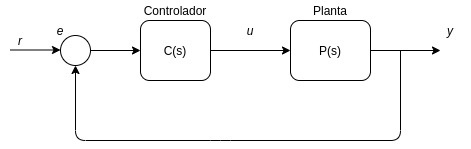
\includegraphics[scale=0.70]{planta.jpg}
%	\caption{Planta PID simples}
%\end{figure}


\postextual

% ----------------------------------------------------------
% Referências bibliográficas
% ----------------------------------------------------------
\bibliography{abntex2-modelo-references}

\phantompart

\printindex

\end{document}
